\section{Subtree}
\subsection*{题意}
给一棵 $n$ 个点的树,对于每个点,求这棵树(作为图)有多少联通子图包含它。
\subsection*{数据范围}
\begin{itemize}
\item $1 \leq n \leq 10^5$
\end{itemize}

\subsection*{题解}

首先我们把这棵树看成以 $1$ 为根的有根树。用$\texttt{son}[i]$ 表示 $i$ 的儿子(们)以及$\texttt{fa}[i]$表示 $i$ 的父亲。

首先注意到树的联通子图必然还是树。对于一个点,我们把所有包含它的子图分成两类,一类以它为根,而另一类的根是它的祖先。假设现在考虑点 $2$。在下面右图中,子图以 $2$ 为根,但在左图中,以 $2$的祖先$1$为根。

\begin{center}
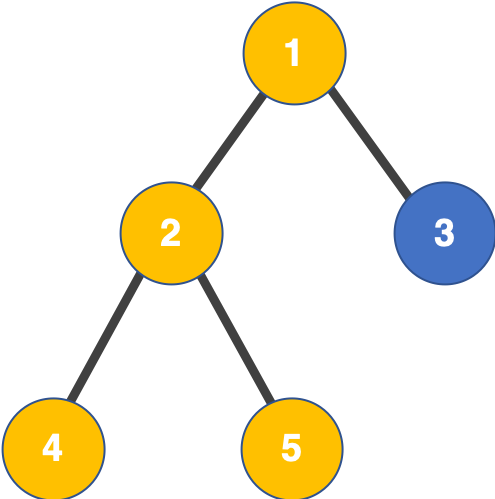
\includegraphics[width=3cm]{./Pics/with_root.png}
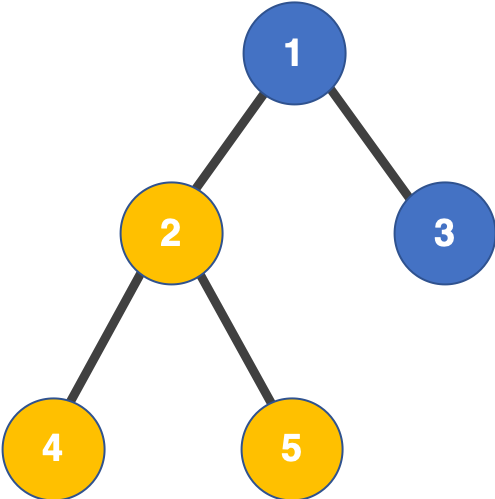
\includegraphics[width=3cm]{./Pics/without_root.png}
\end{center}


首先我们考虑如何计算对于每个点 $i$,以它为根的方案数 $\texttt{dp}[i]$。由于根已经确定,只需要考虑有多少种向下的延伸方式。由于是树,子树间没有联系,所以向各棵子树的延伸方式是独立的,我们只需要把每棵子树的延伸方案数乘起来即可。

对于一棵根为$s$ 的子树,要么完全不进入,要么每种延伸方案恰好和以$s$为根的方案一一对应(把根节点$i$去掉就得到了子树的一个方案)。所以可以得到公式:

$$
\texttt{dp}[i] = \prod_{s\in \texttt{son}[i]} (1+\texttt{dp}[s])
$$

以上只考虑了每个点作为子图的根的情况,这对于全局根节点 $1$ 是足够的,但其他节点总会有向上延伸的情况。由于 $\texttt{dp}[1]$ 恰好等于各个儿子贡献的乘积,不难可以想到我们可以把父亲看作一个特殊的儿子,相当于把父亲旋转成儿子。而父亲方向的贡献应该等于将 $i$ 这个儿子去掉后所剩的方案数,即 $\displaystyle \frac{\texttt{ans}[f]}{dp[i]}$。由于需要在模意义下计算,我们通过前缀积和后缀积的方法避免除法,具体参见代码。





\subsection*{核心代码}
\inputminted[linenos,autogobble]{cpp}{./Code/V.cpp}
\newpage